	\subsection{Opret bruger}
	Dette afsnit vil indeholde en gennem gang af design, grafisk bruger interface og implentering af Opret bruger activityen til android applikationen
	\subsubsection{Design}
	Dette afsnit viser et sekvens diagram over Opret bruger forløbet i android applikationen
	
	\begin{figure} [!ht]
		\begin{center}
			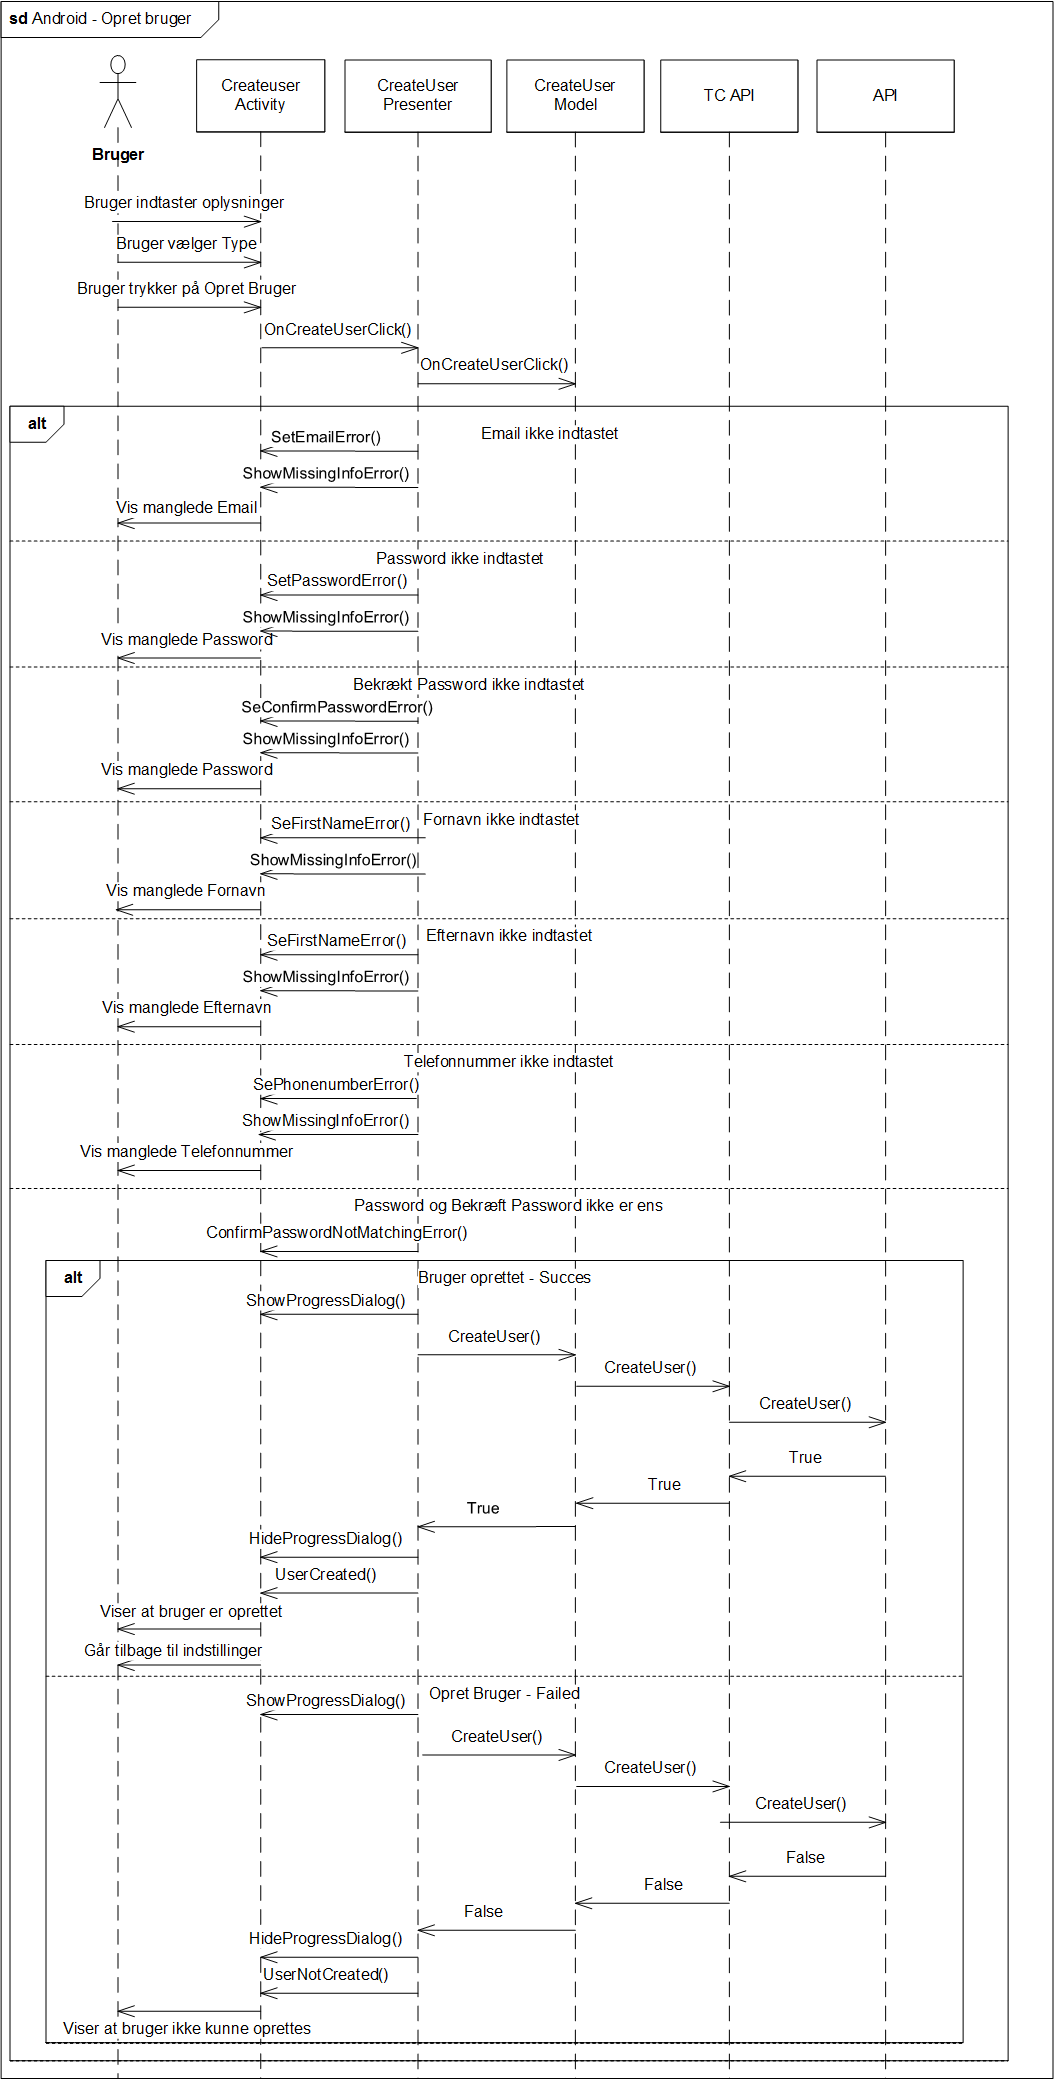
\includegraphics[height=15cm, width=11cm]{Android/Billeder/OpretBrugerSekvens}
		\end{center}
		\caption{Sekvens diagram for opret bruger på android applikationen}
		\label{fig:OpretBrugerSekvens}
	\end{figure}
	
	Klasse relationerne svarer overens men dem i LogInActivity på figur \vref{fig:Klasse diagram for Log Ind Android}. Da opret bruger siden er bygget op omkring MVP på samme måde som log ind siden.
	
	\pagebreak
	
	\subsubsection{Grafisk Bruger Interface}
	Her vises layouttet for Opret Bruger som den ser ud i applikationen.
	\begin{figure}[!ht]
		\begin{center}
			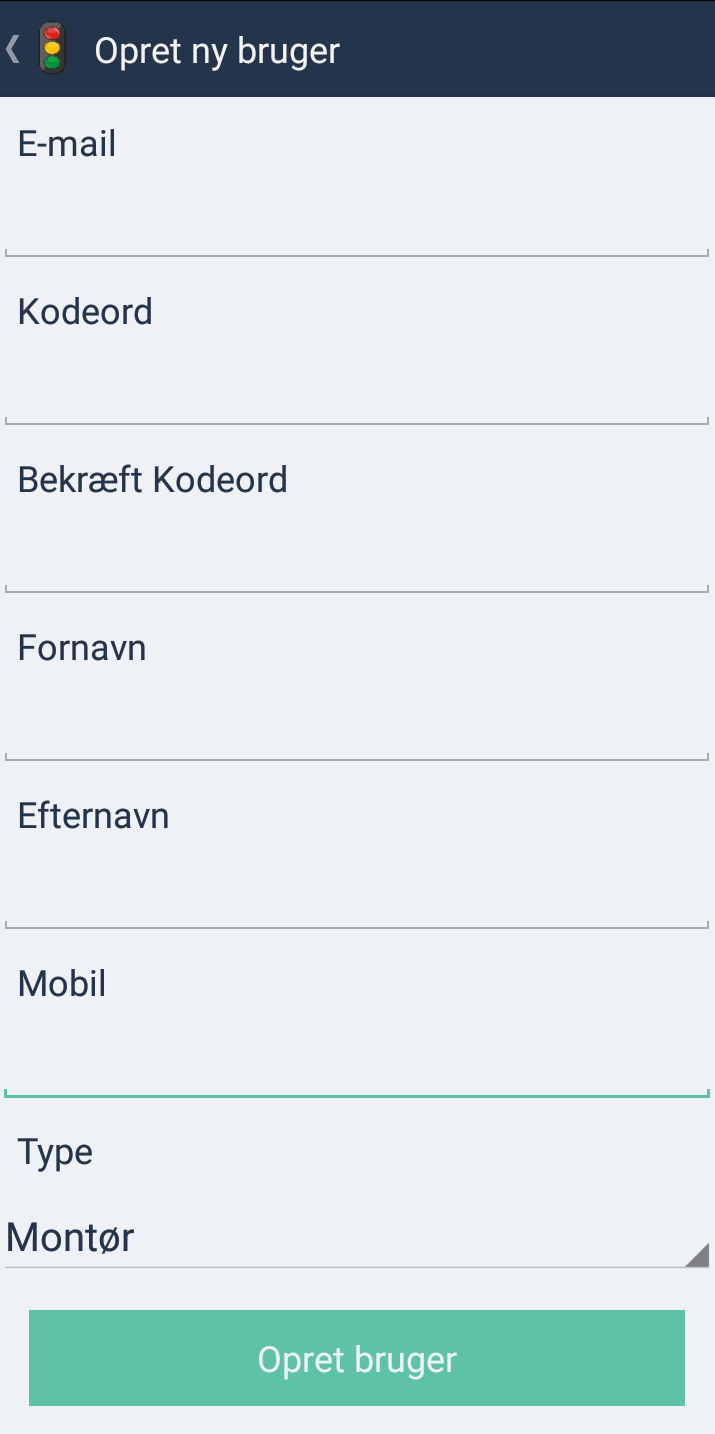
\includegraphics[height=9cm]{Android/Billeder/AndroidOpretbruger}
		\end{center}
		\caption{Traffic Control - Opret Bruger}
		\label{fig: Traffic Control - Opret Bruger}
	\end{figure}
	
	\noindent Opret bruger siden er gjort simpel og nem at arbejde med. Her er lavet felter til alt det info som skal tastes ind om en bruger og til sidst er der lavet en drop down hvor du kan vælge hvilken type bruger det er.	
	\subsubsection{Implementering}
	Når en brugen forsøger at oprette en ny bruger, validerer presenteren at der er indtastet information, inden at informationen bliver sendt videre til modellen. Hvis et felt ikke er udfyldt giver presenteren besked til viewet om at en fejlbesked om dette, skal vises. Hvis alle de påkrævet feltet er fyldt ud bliver et request sendt til API'et, gennem Modellen og DAL-laget.	
	\pagebreak